\chapter{Game Theory}
\section{Taxing Ships in 16th Century Denmark*}\label{sec:denmark}

In the 16th century, foreign ships passing through Øresund, the strait next to Copenhagen, had to make a stop at Helsingør\footnote{The same \href{https://en.wikipedia.org/wiki/Hamlet}{Elsinore} where \textit{Hamlet} takes place} and pay taxes to the Danish Crown based on the value of their cargo (usually 1-5\%). To encourage truth-telling, the Crown reserved the right to buy the entire cargo at the value the captain reports. These are called The Sound Dues. 

Before we dive into the model in \citet{Haan_2012_Taxation}, feel free to \href{https://pbs.twimg.com/media/C1hNo_KUcAAJDQ9.jpg:large}{pause and ponder} for a second. How would you model this situation? What value does the captain report? What is the captain's equilibrium strategy? How much revenue should the Crown expect to collect?

Presuming that you've thought about this a bit yourself already, let's dive into \citet{Haan_2012_Taxation}. First, we see that this is a perfect scenario for game-theoretic modeling. We have two agents: the king and the captain. For simplicity, I will refer to the king as he and the captain as she. The captain has one action: pick a value to report, and the king, upon learning this value, can either choose to tax the ship based on the declared value or buy the cargo. We presume that the king and the captain are both trying to maximize the amount of money they get (here's where the maximization comes in). 

Suppose that the true value of the cargo is $v$, the reported value is $m$ (for message), the tax rate is $t$, and the value of the cargo is the same for the captain and the king.\footnote{The authors dive into the scenario where the cargo is worth more to the captain than the king (because the king has to go through the trouble of seizing the ship and selling the cargo) in the paper. Remember, when you have a situation, it's always a good idea to work through a simple example before generalizing the model.} If the king buys the cargo, he receives $u_K(b) = v - m$; if he chooses to levy a tax, he receives $u_K(t) = mt$. Similarly, we have $u_C(b) = m - v$ and $u_C(t) = -mt$ for the captain. Notice here that the captain plays first, so we have the following game tree:

\begin{figure}[H]
    \caption{Game tree for \citet{Haan_2012_Taxation}}
    \centering
    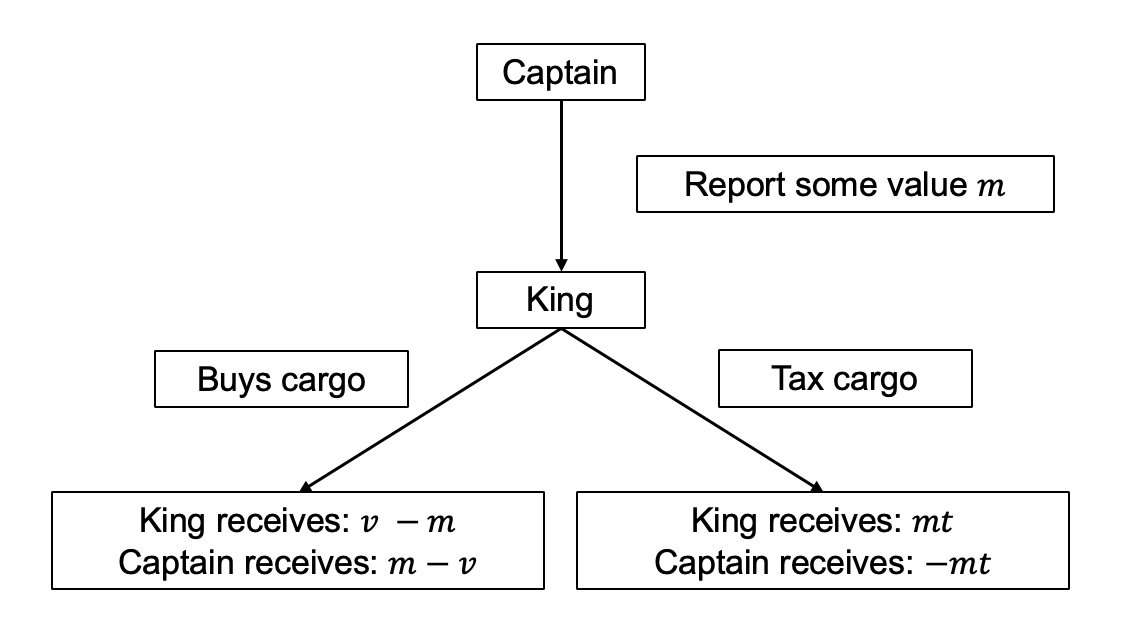
\includegraphics[width = 3.5in]{taxgamertree.png}
\end{figure}

So now we've got a model of the sound dues; let's find the strategies that the king and the captain will play in equilibrium. Why do we care about equilibrium strategy? Well, if we're out of equilibrium, then it means that either the king or the captain can play some other strategy to improve their outcomes. We assume that the agents would have already played an alternative strategy if there is one that improves their payoffs. With that in mind, we introduce the following theorem:

\begin{theorem}
    The king is indifferent between playing buy or tax for any equilibrium message $m$.
\end{theorem}
I will first present an intuitive proof. Suppose that the king prefers to buy the cargo. Then, knowing this, the captain should report a higher value $m$ so that she gets paid more. She should keep on increasing the value until the king is indifferent. Similarly, suppose that the king prefers to tax the cargo, then the captain should report a lower $m$ so she has to pay taxes, and do this until that the king is indifferent. The mathematical proof follows:
\begin{proof}
    Suppose that $v - (1 + t)m > 0$ (i.e., the payoff for the king if he buys the cargo is higher than when he taxes it). Then, there exist some $\epsilon > 0$ such that $m' = m + \epsilon$ and $v - (1 + t)m' > 0$. Thus, the captain can report $m'$ instead of $m$ and gain $m'-v > m - v$, which means that $m$ is not the optimal strategy for the captain, and thus we are not in equilibrium. The proof for when the king prefers taxing the cargo is analogous and is left as an exercise for the reader. 
\end{proof}

Given that the king is indifferent, it follows that the expected payoff that the king gets whether he buys the cargo or not is the same. That is
\begin{align*}
    v - m &= mt \\
    m &= \frac{v}{1 + t}
\end{align*}

We know that as long as the captain plays $m = \frac{v}{1 + t}$, the king would be indifferent. We now check what the king would need to do such that the captain would want to play $m = \frac{v}{1+t}$. Given that the captain has some probability $p(m)$ of playing ``buy", the expected utility of the captain is
\begin{align*}
    EU &= p(m)(m - v) + (1 - p(m))(-tm)
\end{align*}
The captain gets to choose $m$, so we differentiate the equation w.r.t. $m$ and find the optimum
\begin{align*}
    \pd{EU}{m} & = p'(m)(m-v) + p(m) + p'(m)mt -t(1-p(m)) = 0 \\
    & = p'(m)m - p'(m)v + p(m) + p'(m)mt -t + tp(m) = 0
\end{align*}
We know from above that the captain needs to play $m(1+t) = v$ for the king to be indifferent, so we can substitute that in to get
\begin{align*}
    0 & = p'(m)m - p'(m)v + p(m) + p'(m)mt -t + tp(m) \\
    & =  p'(m)m - p'(m)m(1+t)  + p(m) + p'(m)mt -t + tp(m) \\
    & = p(m) -t + tp(m) = 0
\end{align*}
Rearranging gives us
\begin{align*}
    p(m)(1 + t) & = t\\
    p(m) & = \frac{t}{1+t}
\end{align*}
In conclusion, for any given tax rate $t$, the skipper will report $m = \frac{v}{1+t}$, and the king will buy the cargo with probability $\frac{t}{1+t}$ regardless of what was reported. Here, neither player has an incentive to deviate from their current strategy, and thus we have found the Nash equilibrium of the game. 

Since the captain will under-report the true value of their cargo, the mechanism does not induce truth-telling. We see that regardless of what the king plays, he expects to receive $\frac{t}{(1+t)}m$. Thus if the king wants to implement some tax rate $t$, he needs to find tax rate $t^*$ such that $\frac{t^*}{1+t^*} = t$.

More details on this problem can be found in \citet{Haan_2012_Taxation}, but hopefully, this small paragraph gave you a taste of how game-theoretic modeling can be applied to real-life situations. 